\documentclass[12pt]{article}


% packages needed
% \usepackage[english]{babel}
\usepackage{latexsym,amssymb}
\usepackage{xcolor}
\usepackage[pdftex]{graphicx}
\usepackage{amsmath,amsfonts}
\usepackage{multicol} 
\usepackage{pifont}
\usepackage{geometry}

\usepackage{array}
\usepackage{tikz}
\usepackage{pgfplots}

\tikzset{timed/.style=dashed}
\usetikzlibrary{shapes}
\usetikzlibrary{calc}
\usetikzlibrary{backgrounds}
\usetikzlibrary{fit}
\usetikzlibrary{patterns}

\pdfminorversion=4

\renewcommand{\refname}{\sf \large \textbf References}

% \usepackage{enumerate}

\newenvironment{thinitemize}{\itemize\addtolength{\itemsep}{-6pt}}{\enditemize}

\usepackage{paralist}
% \usepackage{algorithmic}
% \usepackage[plain, nothing]{algorithm}

\usepackage{empheq}
\usepackage{multirow}
\usepackage{framed}
\usepackage{fancybox}
\usepackage{wrapfig}

% MYADDITIONS
\usepackage{float}
%\usepackage[caption = false]{subfig}
\usepackage[normalem]{ulem}
 \useunder{\uline}{\ul}{}
 \usepackage{caption}
\usepackage{subfig}
\usepackage{textcomp}

\usepackage{bm} % bold vector with \bm{u}

\usepackage{booktabs}% http://ctan.org/pkg/booktabs
\newcommand{\tabitem}{~~\llap{\textbullet}~~}


\usepackage{epsf}  % read ps

\newenvironment{algorithmUmg}{\begin{small}\begin{tabular}{|l|}\hline}{\\ \hline \end{tabular}\end{small}}

\newcommand{\norm}[2]{\|{#1}\|_{#2}}

\newcommand{\heading}[1]{\large\textsf{\textbf{#1}}}

\newcommand{\dt}{\ensuremath{\Delta t}}
 
% graphics extensions
\DeclareGraphicsExtensions{.jpg,.pdf,.pdftex,.png}
\graphicspath{{./figures/}}
 
% parameters-
\setlength{\pdfpageheight}{594mm}
\setlength{\pdfpagewidth}{420mm}
\setlength{\paperheight}{594mm}
\setlength{\paperwidth}{420mm}
\setlength{\voffset}{-.5in}
% \setlength{\hoffset}{-1.0in}
\setlength{\hoffset}{-0.5in}
\setlength{\evensidemargin}{5mm}
\setlength{\oddsidemargin}{5mm}
\setlength{\topmargin}{0mm}
\setlength{\headheight}{0mm}
\setlength{\headsep}{0mm}
\setlength{\textheight}{624mm}
\setlength{\textwidth}{410mm}
\setlength{\parindent}{0pt}
\setlength{\parskip}{2explus2ex}
\setlength{\fboxsep}{0.01\textwidth}
\setlength{\fboxrule}{0.001\textwidth}
\newlength{\boxwidth}
\setlength{\boxwidth}{0.975\textwidth}
\setlength{\boxwidth}{0.915\textwidth}
\setlength{\columnsep}{1cm}
\setlength{\columnseprule}{0.1pt}
\setlength{\multicolsep}{0cm}
%\setcounter{unbalance}{20}




% font for title of poster
\newcommand{\titlefont}[1]
{\protect{\fontencoding{T1}\fontfamily{pag}\fontseries{b}%
    \fontshape{n}\fontsize{1cm}{1ex}
    \selectfont{#1}}}

\newcommand{\subtitlefont}[1]
{\protect{\fontencoding{T1}\fontfamily{pag}%\fontseries{b}%
    \fontshape{n}\fontsize{0.9cm}{1ex}
    \selectfont{#1}}}
\newcommand{\idn}{\mbox{$1 \hspace{-1.0mm}  {\bf l}$}}


% PAGE HEADINGS
\usepackage{tcolorbox}%

\newcommand{\newpart}[1]
{
    % \tcolorbox{colback=red!5!white,colframe=red!75!black}
    \colorbox[rgb]{0,0,0}
    {\makebox[0.97\columnwidth]
    {\rule[-1.2ex]{0pt}{3.7ex}\partfont{#1}}}
    \bigskip
}
% \colorbox[rgb]{1.0000, 0.9020, 0.4549}
% \tcolorbox{colback=red!5!white,colframe=red!75!black,fonttitle=\bfseries,title=#1}



% Fancy ColorBoxes
 
\newtcolorbox{titlebox}[1]{colback=red!5!white,colframe=red!75!black,fonttitle=\bfseries,title=#1}




% font for headings of pages
\newcommand{\partfont}[1]{{\Large \textsf{\textbf{#1}}}}


% page style
\pagestyle{empty}

% -------------------------------------------------------------------------
\newcommand{\pmat}[1]{\begin{pmatrix}#1\end{pmatrix}} 
\newcommand{\red}[1]{\textcolor{red}{#1}}
\newcommand{\blue}[1]{\textcolor{blue}{#1}}
\newcommand{\brown}[1]{\textcolor{brown}{#1}}
\newcommand{\green}[1]{\textcolor{green}{#1}}
\newcommand{\purple}[1]{\textcolor{purple}{#1}}
\newcommand{\gray}[1]{\textcolor{gray}{#1}}

\newcommand{\integral}[1]{\int_{t_0}^{t_N} {#1} \, dt}
\newcommand{\fsum}[3]{\sum_{#1}^{#2}{#3}} 
\newcommand{\pder}[2]{\frac{\partial #1}{\partial #2}}
\newcommand{\dder}[2]{\frac{d #1}{d #2}}

\def \R{\bb{R}}\def \C{\bb{C}}\def \Z{\bb{Z}}\def \N{\bb{N}}
\def \a{{\bf a}}
\def \b{{\bf b}}
\def \c{{\bf c}}
\def \d{{\bf d}}
\def \e{{\bf e}}
\def \f{{\bf f}}
\def \g{{\bf g}}
\def \k{{\bf k}}
\def \m{{\bf m}}
\def \n{{\bf n}}
\def \p{{\bf p}}
\def \q{{\bf q}}
\def \r{{\bf r}}
\def \s{{\bf s}}
\def \t{{\bf t}}
\def \u{{\bf u}}
\def \v{{\bf v}}
\def \w{{\bf w}}
\def \x{{\bf x}}
\def \y{{\bf y}}
\def \h{{\bf h}}
\def \z{{\bf z}}
\def \rh{{\alert{h}}}
\def \M{{\cal M}}
\def \F{{\cal F}}
\def \L{{\cal L}}
\def \R{{\bf R}}
\def \J{{\cal J}}
\def\0{{\bf 0}}
\def\p{{\bf{g}}}
\def \blambda{{\boldsymbol{\lambda}}}
%--------------------------------------------------------------------------
%%%%%%%%%%%%%%%%%%%%%%%%%%%%%%%
%%%%%%%%%%%%%%%%%%%%%%%%%%%%%%%

\def\minim{\mathop{\hbox{\rm minimize}}}
\def\minimize#1{{\displaystyle\minim_{#1}}}
\def\subject{\mbox{\rm subject to}}
\def\myobj{J}
\def\problemI#1#2#3#4{%\fbox
   {\begin{tabular*}{0.3\textwidth}
    {@{}l@{\extracolsep{\fill}}l@{\extracolsep{6pt}}l@{\extracolsep{\fill}}c@{}}
      #1 & $\minimize{#2}$ & $#3$ & $ $ \\[5pt]
         & $\subject$      & $#4$ & $ $
    \end{tabular*}}}

\def\problemII#1#2#3#4#5{%\fbox
   {\begin{tabular*}{0.3\textwidth}
    {@{}l@{\extracolsep{\fill}}l@{\extracolsep{6pt}}l@{\extracolsep{\fill}}c@{}}
      #1 & $\minimize{#2}$ & $#3$ & $ $ \\[5pt]
         & $\subject$      & $#4$ & $ $ \\[5pt]
         & & $#5$ & $ $
    \end{tabular*}}}

\def\problemIII#1#2#3#4#5#6{%\fbox
   {\begin{tabular*}{0.3\textwidth}
    {@{}l@{\extracolsep{\fill}}l@{\extracolsep{6pt}}l@{\extracolsep{\fill}}c@{}}
      #1 & $\minimize{#2}$ & $#3$ & $ $ \\[5pt]
         & $\subject$      & $#4$ & $ $ \\[5pt]
         & & $#5$ & $ $ \\[5pt]
         & & $#6$ & $ $ 
    \end{tabular*}}}


% pgfplots
\usepackage{tikz}
\usepackage{pgfplots}
\usepackage{pgfplotstable}

% Colored tables
\pgfplotstableset{
  discard if equal/.style = {
    preproc cell content/.code={
      \ifdim##1pt=#1pt
        \pgfkeyssetvalue{/pgfplots/table/@cell content}{}
      \fi
    }
  },
  color cells/.style = {
    postproc cell content/.code={
      \pgfkeyssetvalue{/pgfplots/table/@cell content}{\cellcolor{#1}##1}
    }
  }
}



% tabularx environment
\usepackage{tabularx}
\newcolumntype{C}{>{\centering\arraybackslash}X}
\usepackage{graphicx}

% Colors custom
%\definecolor{mycolor1}{HTML}{CA0020}
%\definecolor{mycolor2}{HTML}{F4A582}
%\definecolor{mycolor3}{HTML}{F7F7F7}
%\definecolor{mycolor4}{HTML}{92c5de}
%\definecolor{mycolor5}{HTML}{0571b0}

%  Blocks 
\usepackage{tcolorbox}

\tcbuselibrary{skins,breakable}
\usetikzlibrary{shadings,shadows}


\newenvironment{myblock}[1]{%
    \tcolorbox[beamer,%
    noparskip,breakable,
    colback=black!05!white,colframe=white!20!black,%
    colbacklower=blue,%
    title=#1]}%
    {\endtcolorbox}

\newenvironment{defblock}[1]{%
    \tcolorbox[beamer,%
    noparskip,breakable,
    colback=black!05!white,colframe=white!20!black,%
    colbacklower=blue,%
    title=#1]}%
    {\endtcolorbox}



% Bold vector
\newcommand{\vect}[1]{\boldsymbol{#1}} 


% Math shortcuts
\newcommand{\1}{\mathbf{1}}
\def\subject{\mbox{\rm subject to}}
\def\minim{\mathop{\hbox{\rm minimize}}}
\def\minimize#1{{\displaystyle\minim_{#1}}}
\DeclareMathOperator*{\argmin}{argmin}




\usepackage{siunitx}
\usepackage{booktabs}
\usepackage{colortbl}

% Algorithm Pseudocode
\usepackage{algorithm}
%\usepackage{algorithmic}
\usepackage{algpseudocode}

\renewcommand{\algorithmicrequire}{\textbf{Input:}}
\renewcommand{\algorithmicensure}{\textbf{Output:}}
\algnewcommand{\algorithmicand}{\textbf{ and }}
\algnewcommand{\algorithmicor}{\textbf{ or }}
\algnewcommand{\OR}{\algorithmicor}
\algnewcommand{\AND}{\algorithmicand}


% Min, Max, RCCut
\def\Min{\text{min}}
\def\Max{\text{max}}
\def\RCCut{\text{RCCut}}







\begin{document}

%\BgThispage % activate background

\fbox{
\parbox{0.9972\boxwidth}{
\hspace*{-.3cm}
\begin{minipage}{0.3\textwidth}
  \begin{tikzpicture}
    %\node [anchor=north] (label) at (0,0)
    %{\includegraphics[width=\textwidth]{images/eth_logo_black.pdf}};
    \node [anchor=south] (label) at (0,0.1) {\includegraphics[width=0.75\textwidth]{figures/usi_inf.jpg}};
%    \node [anchor=south] (label) at (0,5.5) {\includegraphics[scale=0.4]{figures_2/bern}};
  \end{tikzpicture}
\end{minipage}
\hspace*{0.02\textheight}
\begin{minipage}{0.58\textwidth}
  \titlefont{Particle Simulations with OpenACC: Speedup and Scaling}\\[0.4cm]
\Huge{Samuel A. Cruz Alegría, Alessandra M. de Felice, Hrishikesh R. Gupta}\\
\end{minipage}
}
}
% Information about openacc


% ======================================== %
% General introduction to OpenACC
% ======================================== %

\fbox{
  \parbox{1.001\boxwidth}{
    \setlength{\fboxsep}{0.005\textwidth}
    \setlength{\fboxrule}{0.00125\textwidth}
    
    \raggedcolumns
    \begin{multicols}{2}
         
    \vbox to 0.2\textheight {%
    \newpart{\color{white}{\textbf{OpenACC}}}

% \centering

% \vspace{-6.0cm}

\begin{minipage}{.45\columnwidth}
\begin{itemize}
    \item[] For a graph $\mathcal{G}(V,E)$ with $n$ vertices and $m$ edges:
    \item Incidence matrix: $\vect{A} \in \R^{m \times n}$, 
    \item Graph Laplacian matrix: $\vect{L} \in \R^{n \times n}$,
    \item Vertex potentials: 
    $
        x_i = 
        \left\{
        \begin{array}{cc}
        1 \,,\quad i \in V_k, \\
        0 \,,\quad i \in \overline{V_k}.
    \end{array}
    \right.
    $
\end{itemize}

\begin{align*}
\displaystyle
\vect{A}
\scriptscriptstyle
   &= 
    \begin{bmatrix*}[r]
    1 & -1 & 0 & 0 \\
    0 & 1 & -1 & 0 \\
    0 & 0 & 1 & -1 \\
    0 & 1 & 0 & 1 \\
    -1 & 0 & 0 & 1 
  \end{bmatrix*}, 
\displaystyle  
\vect{L} 
   = \vect{A}^T \vect{A} = 
   \scriptscriptstyle
    \begin{bmatrix*}[r]
    2 & -1 & 0  & -1  \\
   -1 & 3  & -1 & -1  \\
    0 & -1 & 2  & -1 \\
    -1 & -1  & -1 & 3 
  \end{bmatrix*}
\end{align*}

\end{minipage}
\hfill
\begin{minipage}{.45\columnwidth}

\begin{figure}[H]
\includegraphics[width=0.94\columnwidth]{figures/simple_graph_small_bold.png}
\end{figure}
\end{minipage}

\vspace{0.2cm}

\begin{myblock}{}
\centering
Calculate an edge separator using the Fiedler eigenvector of $\mathbf{L}\in\R^{n \times n}$.
\end{myblock}


\begin{minipage}{.58\columnwidth}
\centering
\vspace{+0.5cm}
\begin{defblock}{
\centering
2-Laplacian partitioning
}
\centering
\begin{align*}
 \min_{V_k \subset V} \frac{\|\vect{A}\hat{\x}\|_2^2}{\|\hat{\x}\|_2^2}
&\approx
  \min_{\vect{x} \in \mathbb{R}^n} \frac{\|\vect{A}\x\|_2^2}{\|\x\|_2^2}     
    = \min_{\vect{x} \in \mathbb{R}^n} \frac{ \x^\top \vect{L}\x}{\x^\top \x} = \lambda^{(2)}_i  \\ 
 &\subject{\ } \1^\top \x  = 0
\end{align*}

\end{defblock}

\vspace{+0.5cm}

\begin{defblock}{ 
\centering
p-Laplacian partitioning,
}
\centering
\begin{align*}
 \min_{V_k \subset V} \frac{\|\vect{A}\hat{\x}\|_p^p}{\|\hat{\x}\|_p^p}
\approx&
  \min_{\vect{x} \in \mathbb{R}^n} \frac{\|\vect{A}\x\|_p^p}{\|\x\|_p^p} 
    = \min_{\x \in \R^n} \frac{ (\vect{A} \x)^\top \phi_p (\vect{A} \x) } {\x^\top \phi_p( \x)} = \lambda^{(p)}_i \\ 
 &\subject{\ } \1^\top \phi_p(\x)  = 0
\end{align*}

\end{defblock}

\end{minipage}
\hfill
\begin{minipage}{.42\columnwidth}
\centering

\centering
% \vspace{-1.6cm}
\textbf{Feasible Projection}\\
% \vspace{+0.2cm}
\begin{equation*}
\widehat{\x} = \x - \frac{\1^\top\x}{n}
\end{equation*}

\vspace{+1.2cm}

\centering
\begin{align*}
\phi_p(x_i) &= |x_i|^{p-2}x_i, \; i = 1, \ldots, n \\
\phi_p^{-1}(x_i) &= |x_i|^{\frac{1}{p-1}} \text{sign}(x_i)    
\end{align*}

\centering
\vspace{-0.6cm}
\begin{align*}
\widehat{\x}_p &=  \phi_p^{-1} \left(\phi_p(\x) - \frac{\1^\top \phi_p(\x)}{n} \right)
\end{align*}


\end{minipage}

%\vfill
%%% stop editing here
\columnbreak
} % end vbox


% ======================================== %
%     Examples of OpenACC
% ======================================== %

%\vspace{1cm}
\columnbreak
\newpart{\color{white}{\textbf{OpenACC Examples and Uses}}}


\begin{figure}[H]
    \centering % <-- added

  \includegraphics[width=0.32\columnwidth]{figures/1354_METIS2.png}
  \includegraphics[width=0.32\columnwidth]{figures/1354_PLAPMETIS2.png}
  \includegraphics[width=0.32\columnwidth]{figures/1354_PLAPKaHIP2.png}
\end{figure}

\begin{center}
\begin{table}[H]
\scalebox{0.8}{
% \colorbox{lightgray}{%
  \centering
  \renewcommand{\arraystretch}{1.4}
\pgfplotstabletypeset[
        columns/Case/.style={column name=Case,string type,column type=l},
        columns/Nodes/.style={int detect,column type=r},
        columns/Edges/.style={int detect,column type=r},
        columns/Metis/.style={column name=\textbf{METIS},string type,column type=c},
        columns/Metis-imbal/.style={column name=$b_r^2$(\%),string type,column type=c},
        columns/pLapMetis/.style={column name=\textbf{p-Lap(METIS\%)}, string type,column type=c},
        columns/pLapMetis-imbal/.style={column name=$b_r^2$(\%), string type,column type=c},
        columns/KaHIP/.style={column name=KaHIP,string type,column type=c},
        columns/KaHIP-imbal/.style={column name=$b_r^2$(\%),string type,column type=c},
        columns/pLapKaHIP/.style={column name=\textbf{p-Lap(KaHIP\%)}, string type,column type=c},
        columns/pLapKaHIP-imbal/.style={column name=$b_r^2$(\%), string type,column type=c},
        every head row/.style={
        before row=\toprule,after row=\midrule},
        every last row/.style={
        after row=\bottomrule},
columns={Case,Nodes,Edges,Metis,Metis-imbal,pLapMetis,pLapMetis-imbal,KaHIP,KaHIP-imbal,pLapKaHIP,pLapKaHIP-imbal},
]{Case1354.dat}
}
% }
\end{table}
\end{center}

\vspace{-1.5cm}

\begin{figure}[H]
    \centering % <-- added
  \includegraphics[width=0.4\columnwidth]{figures/6495_KaHIP.png} 
  \hspace{1.5cm}
  \includegraphics[width=0.4\columnwidth]{figures/6945_PLAPKaHIP.png}
\end{figure}

\begin{table}[H]
\scalebox{0.8}{
% \colorbox{lightgray}{%
  \centering
  \renewcommand{\arraystretch}{1.4}
\pgfplotstabletypeset[
        columns/Case/.style={column name=Case,string type,column type=l},
        columns/Nodes/.style={int detect,column type=r},
        columns/Edges/.style={int detect,column type=r},
        columns/Metis/.style={column name=METIS,string type,column type=c},
        columns/Metis-imbal/.style={column name=$b_r^2$(\%),string type,column type=c},
        columns/pLapMetis/.style={column name=p-Lap(METIS\%), string type,column type=c},
        columns/pLapMetis-imbal/.style={column name=$b_r^2$(\%), string type,column type=c},
        columns/KaHIP/.style={column name=\textbf{KaHIP},string type,column type=c},
        columns/KaHIP-imbal/.style={column name=$b_r^2$(\%),string type,column type=c},
        columns/pLapKaHIP/.style={column name=\textbf{p-Lap(KaHIP\%)}, string type,column type=c},
        columns/pLapKaHIP-imbal/.style={column name=$b_r^2$(\%), string type,column type=c},
        every head row/.style={
        before row=\toprule,after row=\midrule},
        every last row/.style={
        after row=\bottomrule},
columns={Case,Nodes,Edges,Metis,Metis-imbal,pLapMetis,pLapMetis-imbal,KaHIP,KaHIP-imbal,pLapKaHIP,pLapKaHIP-imbal},
]{Case6495.dat}
}
% }
\end{table}
  
  
\end{multicols}}}



% ======================================== %
%    Particle Simulations
% ======================================== %

\fbox{
  \parbox{0.9972\boxwidth}
  {
    \setlength{\fboxsep}{0.005\textwidth}
    \setlength{\fboxrule}{0.00125\textwidth}
    
     \raggedcolumns
      \begin{multicols}{2}

\vbox{

\newpart{\color{white}{Particle Simulations}}

\begin{minipage}{.49\columnwidth}


\begin{algorithm}[H]
\caption{$p$-Laplacian Bisection}
{\fontsize{10}{20}\selectfont
\begin{algorithmic}[1] 
\Require $\x_0$ \Comment{METIS or KaHIP bisection}
\Ensure  $\x_p^\Min$ \Comment{$p$-Laplacian bisection}
\Function{pLaplacian}{$\vect{A}, \x_0, b^{\text{max}}, \beta, \text{max\_it}$}
  \State $\color{purple}{\displaystyle r_c^\Min \gets \RCCut(\x_0)}$
  \State $p=2, \quad \displaystyle \x= \x_0$
  \For{k=0:max\_it}
  \State  $\displaystyle p_k = {1 + e^{-\beta k/\text{max\_iters}} }$
    \State $\x_k^{\text{min}} \gets \text{pLaplacianDescent}(\vect{A}, p_k)$ 
  \EndFor
  \State \Return {$\x_p^\Min$}
  \EndFunction
\end{algorithmic}
}
\end{algorithm}

\end{minipage}
\hfill
\begin{minipage}{.49\columnwidth}
% 
\begin{algorithm}[H]
\caption{$p$-Laplacian Descent}
{\fontsize{10}{12}\selectfont
\begin{algorithmic}[1]
\Require $\x_0$ \Comment{approximation of the $p$-eigenvector}
\Ensure  $\x_p^\Min$ \Comment{$p$-Laplacian bisection}
\Function{pLaplacianDescent}{$\vect{A}, \x_0, p$}
   	\While{not converged}
      \State $\color{purple}{\displaystyle \x \gets \widehat{\x}_p}$
      \State $r_c = \text{RCCut}(\x)$ 
      \State $\color{purple}{b_r = \text{ImBal}(\x)}$
    
   	  \If{$r_c < r_c^\Min$ \AND $b_r < b_r^\Max$}
        \State $\x^\Min_p \gets \x$
        \Comment{save best solution}
        \State $r_c^\Min \gets r_c$
        \Comment{and minimum cut}
      \EndIf
      \State $\displaystyle \g  \gets \nabla f(\x)$
      \State $\displaystyle \alpha \gets \argmin_\alpha f\left(\phi^{-1}_p \left( \x - \alpha \g \right) \right)$
      \State $\displaystyle \x \gets \phi^{-1}_p \left( \x - \alpha \g \right)$
	\EndWhile
  \State \Return {$\x^\Min_p$}
\EndFunction
\end{algorithmic}
} % spacing
\end{algorithm}
\end{minipage}

\begin{itemize}
\item Ratio Cheeger cut: $ \displaystyle
\text{RCCut}(V_k,\overline{V}_k) = \frac{\text{cut}(V_k,\overline{V}_k)}{\min\{|V_k|,|\overline{V}_k|\}}, \;\; \text{with} \;\; \text{cut}(V_k,\overline{V}_k) = \|\vect{A}\x\|_p^p.
$
\item Node imbalance: $ \displaystyle
b_r^2 = 
\frac{ \big |  |V_2| - |\overline{V}_2| \big|}{|V|}.
$
\item Reduced computational complexity: $\displaystyle O(n^3) \rightarrow O(m)$. 
\end{itemize}





} % vbox


 \columnbreak

% ======================================== %
%         Particle Simulations integrated with OpenACC - Performance results
% ======================================== %

\newpart{\color{white}{ Particle Simulations Integrated with OpenACC}}
\vbox to 0.1999\textheight
{
  \raggedcolumns
  \setlength{\columnseprule}{0.pt}
  
\vspace{+0.5cm}

\begin{itemize}
    \item Consistent and valid improvement over a METIS or KaHIP partition.
    \item The level of improvement achieved depends on the structure of the graph in question and the optimality or near optimality of the original cut
\end{itemize}
 From a total of 186 graphs initialized with a METIS cut, improvements over 10\% were observed for 47.3\% of them, while for the 102 graphs initialized with a KaHIP partition improvements over 10\% were observed for 15.7\% of them.

% \input{CollectiveMETIS.tex}

% \input{CollectiveKaHIP.tex}

\centering
\vspace{+0.9cm}
\includegraphics[width=0.96\columnwidth]{figures/concentrated_2.png}


 
} % end vbox


\end{multicols}
   } % end parbox

} % end fbox

% ======================================== %
% Parallel p-Laplacian Graph Partitioning
% ======================================== %
\fbox{
  \parbox{0.9972\boxwidth}{
    \setlength{\fboxsep}{0.005\textwidth}
    % \setlength{\fboxsep}{0.505\textwidth}
    \setlength{\fboxrule}{0.00125\textwidth}
    % \setlength{\fboxrule}{0.10125\textwidth}
    % --------------------------------------------------------------------------
    \setlength{\columnwidth}{1.02\linewidth}
    \newpart{\color{white}{Parallel Particle Simulations}}
\vbox to 0.182\textheight {%

%% start editing here

	 \raggedcolumns
	 
		 	\setlength{\columnseprule}{0.pt}
			
   			 \begin{multicols}{3}

				\vfill
% ======================================== %
%               Motivation - ICS and Master Programme
% ======================================== %
\begin{center}
\heading{Motivation - ICS and Master Programme}
\end{center}

\begin{center}
\includegraphics[width=0.66\columnwidth]{figures/Piz-Daint.png}    
\end{center}

The bisection of a finite-element mesh on an XC50 compute node of Piz Daint at the Swiss National Supercomputing Centre indicates that the $p$-Laplacian algorithm is suitable for parallel computation and is able to utilize the capabilities of modern computer hardware.

\begin{table} [H]
\renewcommand{\arraystretch}{1.3}
\caption*{15,360,000 elements, 2,618,021 nodes}
\vspace{-0.3cm}
\scalebox{0.95}{
\centering
\pgfplotstabletypeset[
        columns/CPU/.style={string type,column type=c},
        columns/FLOPS/.style={column name=Peak FLOPS,string type,column type=c},
        columns/MEM/.style={string type,column type=c, column name=(Peak MEM.)},
        columns/TIME/.style={column name=Elapsed time (s),string type,column type=c},
        every head row/.style={
        before row=\toprule,after row=\midrule},
        every last row/.style={
        after row=\bottomrule},
columns={CPU,FLOPS,MEM,TIME},
]{Motivation.dat}
} % scalebox
\end{table}


\centering
% \begin{figure}
% \begin{tabularx}{\textwidth}{CCC}
%     % empty top left
%     &   \includegraphics[width=0.33\columnwidth]{figures/Piz-Daint.png}
%     &   
%     % empty top right 
%     \\
%     % [-3ex]
%     % \vspace{-1.8cm}
% \includegraphics[width=0.33\columnwidth]{figures/intel-xeon.jpg}
%     &   
%     % empty bottom center
%     & 
%     % \vspace{-1.8cm}
%     \includegraphics[width=0.33\columnwidth]{figures/nvidia_tesla.jpg}
% \end{tabularx}
% % \end{figure}


%----------------------------------------------------------------------------
\columnbreak

% ======================================== %
%               ICS Cluster
% ======================================== %
\begin{center}								
\heading{ICS Cluster}  
\end{center}
 


\begin{table} [H]
  \renewcommand{\arraystretch}{1.3}
%   \caption*{15,360,000 elements, 2,618,021 nodes}
  \vspace{-0.3cm}
%   \scalebox{0.65}{
  \centering
\pgfplotstabletypeset[
        columns/Method/.style={string type,column type=c},
        columns/EdgeCut/.style={column name=edgecut,int detect,column type=r},
        columns/PercentEdgeCut/.style={string type,column type=c, column name=(METIS\%)},
        columns/MaxWeight/.style={column name=$\displaystyle \max_{i\le128}{\big|V^{128}_i\big|}$,int detect,column type=r},
        columns/Imbal/.style={column name=$b_r^{128}$(\%),string type,column type=r},
        every head row/.style={
        before row=\toprule,after row=\midrule},
        every last row/.style={
        after row=\bottomrule},
columns={Method,EdgeCut,PercentEdgeCut,MaxWeight,Imbal},
]{Hybrid.dat}
% }%scalebox
\end{table}

\vspace{+0.7cm}

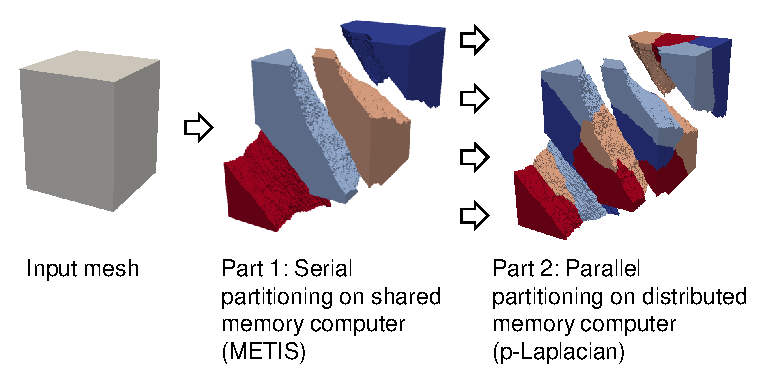
\includegraphics[width=0.99\columnwidth]{figures/hybrid}

                      
% ======================================== %
%             Visuals and Performance
% ======================================== %
\columnbreak
%----------------------------------------------------------------------------
                                 
\begin{center}
 \heading{Visualisation and Performance}
\end{center}
The elapsed time is measured on SGI UV300 for METIS and part 1 of the hybrid method, and P100 GPUs on Piz Daint XC50 nodes. The largest finite-element mesh partitioned, consisting of 1.9 billion tetrahedra, corresponds to an application using 77\% of the Piz Daint system (4,096 compute nodes).
 \\
 \vspace{+1cm}
 \includegraphics[width=0.90\columnwidth]{figures/scalability.png}
% \includegraphics[width=0.30\textwidth]{figures_2/speed}


 %\vfill
%				%--------------------------------------------------------------------------
%  \vspace{1mm}
%\vfill
\end{multicols}}

} % end vbox
%----------------------------------------------------------------------------

}



\,\, T. Simpson, D. Pasadakis, D. Kourounis, K. Fujita, T. Yamaguchi, T. Ichimura, and O. Schenk, ``Balanced graph partition refinement using the graph p-Laplacian," in {\it Proceedings of the ACM Platform for \\ Advanced Scientific Computing Conference,} ser. PASC'18, July 2018, accepted, in press. (acceptance rate: 21.5 \%).


%%%%%%%%%%%%%%%%%%%%%%%%%%%%%%%%%%%%%%%%%%%%%%%%%%%%%%%%%%%%
%  END
%%%%%%%%%%%%%%%%%%%%%%%%%%%%%%%%%%%%%%%%%%%%%%%%%%%%%%%%%%%%
\end{document}
